\chapter{Lec 07 - 08 - Linear Regression II}

\section{$R^2$ Statistic}
The $R^2$ statistic provides a measure of lack of fit of the linear model to the data. It takes the form of a proportion, the proportion of variance explained, and so it always takes on a value between 0 and 1, and is independent of the scale of $Y$. To calculate $R^2$, we use the formula
\[R^2 = \frac{TSS - RSS}{TSS} = 1 - \frac{RSS}{TSS}\]
where
\[TSS = \sum_{i=1}^n (y_i - \bar{y})^2 \quad RSS = \sum_{i=1}^n (y_i - \hat{y}_i)^2\]
TSS (total sum of squares) measures the total variance in the response $Y$, and can be  thought of as the amount of variability inherent in the response before the regression is performed \footnote{note that TSS corresponds to the best prediction we can do without having features}. In contrast, RSS measures the amount of variability that is left unexplained after performing the regression. Hence, TSS - RSS measures the amount of variability in the response that is explained (or removed) by performing the regression, and $R^2$ measures the proportion of variability in $Y$ that can be explained using $X$.\\\\
An $R^2$ statistic that is close to 1 indicates that a large proportion of the variability in the response has been explained by the regression. A number near 0 indicates that the
regression did not explain much of the variability in the response; this might occur because the linear model is wrong, or the inherent error $\sigma^2$ is high, or both.\\\\
This can also be seen by looking at the formulas of TSS and RSS. In particular, RSS can be written as
\[RSS = \sum_{i=1}^n (y_i - (\hat\beta_0 + \hat\beta_1 x_i))^2\]
Recall that $\hat\beta_0$ and $\hat\beta_1$ are estimated in the following way:
\[
\begin{split}
    \hat{\beta}_1 = & \frac{\sum_{i=1}^n (x_i - \overline{x}) (y_i - \overline{y})}{\sum_{i=1}^n (x_i - \overline{x})^2} \\
    \hat{\beta}_0 = & \overline{y} - \hat{\beta}_1 \overline{x}
\end{split}
\]
Then, if $\hat\beta_1 = 0$, which means no correlation between $X$ and $Y$, the RSS formula becomes
\[RSS = \sum_{i=0}^n (y_i - \hat\beta_0)^2 = \sum_{i=0}^n (y_i - \overline{y})^2 = TSS\]
The $R^2$ statistic is a measure of the linear relationship between $X$ and
$Y$. Recall that correlation, defined as
\[\text{Cor}(X,Y) = \frac{\sum_{i=1}^n (x_i - \overline{x})(y_i - \overline{y})}{\sqrt{\sum_{i=1}^n (x_i - \overline{x})^2} \sqrt{\sum_{i=1}^n (y_i - \overline{y})^2}}\]
It can be shown that in the \textit{simple linear regression} setting, $R^2 = \text{Cor}(X,Y)^2$. In other words, the squared correlation and the $R^2$ statistic are identical. However, in the multiple linear regression problem, in which we use several predictors simultaneously to predict the response, this equality does not hold.

\section{Multiple Linear Regression}
Simple linear regression is a useful approach for predicting a response on the basis of a single predictor variable. However, in practice we often have more than one predictor. One option is to run three separate simple linear regressions, each of which uses a different advertising medium as a predictor. However, this approach is not entirely satisfactory.\\\\
Instead of fitting a separate simple linear regression model for each predictor, a better approach is to extend the simple linear regression model so that it can directly accommodate multiple predictors. We can do this by giving each predictor a separate slope coefficient in a single model. In general, suppose that we have $p$ distinct predictors. Then the multiple linear regression model takes the form
\[Y = \beta_0 + \beta_1 X_1 + \beta_2 X_2 + ... + \beta_p X_p + \epsilon\]
We interpret $\beta_j$ as the average effect on $Y$ of a one unit increase in $X_j$, holding all other predictors fixed. Given estimates $\hat\beta_0, \hat\beta_1, . . . \hat\beta_p$, we can make predictions using the formula
\[\hat{y} = \hat\beta_0 + \hat\beta_1 x_1 + \hat\beta_2 x_2 + ... + \hat\beta_p x_p\]
As we did for the simple linear model, we estimate $\beta_0, \beta_1, . . . , \beta_p$ as the values that minimize the sum of squared residuals $RSS = \sum_{i=1}^n (y_i - \hat{y}_i)^2$.
This is done using standard statistical software. The values $\hat\beta_0, \hat\beta_1, . . . \hat\beta_p$ that minimize RSS are the multiple least squares regression coefficient estimates.

\subsection{Example: Qualitative Predictors}
In our discussion so far, we have assumed that all variables in our linear
regression model are quantitative. But in practice, this is not necessarily
the case; often some predictors are qualitative.\\\\
Suppose that we wish to investigate differences in credit card balance between males and females. If a qualitative predictor (also known as a \textit{factor}) only has two \textit{levels}, or possible values, then incorporating it into a regression model is very simple. We simply create an indicator or dummy variable that takes on two possible numerical values. For example, based on the gender variable, we can create a new variable that takes the form
\[
x_i = 
\begin{cases}
    1 & \text{if $i$-th person is female}\\
    0 & \text{if $i$-th person is male}
\end{cases}
\]
and use this variable as a predictor in the regression equation. This results
in the model
\[y_i = \beta_0 + \beta_1 x_i + \epsilon_i = 
\begin{cases}
    \beta_0 + \beta_1 + \epsilon_i & \text{if $i$-th person is female}\\
    \beta_0 + \epsilon_i & \text{if $i$-th person is male}
\end{cases}
\]
Now $\beta_0$ can be interpreted as the average credit card balance among males, $\beta_0 + \beta_1$ as the average credit card balance among females, and $\beta_1$ as the average difference in credit card balance between females and males.
\begin{center}
    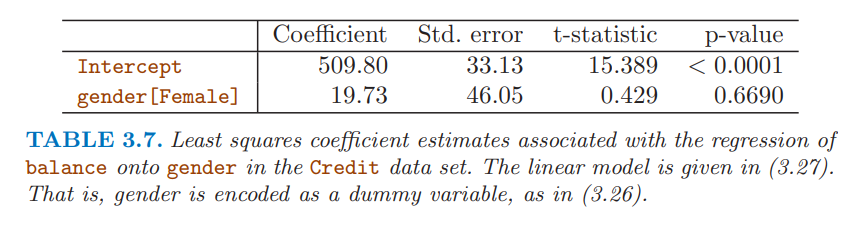
\includegraphics[scale=0.8]{images/dummy_var_1.png}
\end{center}
In the table above we can see that the average credit card debt for males is
estimated to be \$509.80, whereas females are estimated to carry \$19.73 in
additional debt for a total of \$509.80 + \$19.73 = \$529.53. However, we
notice that the p-value for the dummy variable is very high. This indicates
that there is no statistical evidence of a difference in average credit card balance between the genders.\\\\
The decision to code females as 1 and males as 0 is arbitrary, and has no effect on the regression fit, but does alter the interpretation of the coefficients.  If we had coded males as 1 and females as 0, then the estimates for $\beta_0$ and $\beta_1$ would have been 529.53 and -19.73, respectively, leading once again to a prediction of credit card debt of \$529.53 - \$19.73 = \$509.80 for males and a prediction of \$529.53 for females. Alternatively, instead of a 0/1 coding scheme, we could create a dummy variable
\[
x_i = 
\begin{cases}
    1 & \text{if $i$-th person is female}\\
    -1 & \text{if $i$-th person is male}
\end{cases}
\]
and use this variable in the regression equation. This results in the model
\[y_i = \beta_0 + \beta_1 x_i + \epsilon_i = 
\begin{cases}
    \beta_0 + \beta_1 + \epsilon_i & \text{if $i$-th person is female}\\
    \beta_0 - \beta_1 +  \epsilon_i & \text{if $i$-th person is male}
\end{cases}
\]
Now $\beta_0$ can be interpreted as the overall average credit card balance (ignoring the gender effect), and $\beta_1$ is the amount that females are above the average and males are below the average. It is important to note that the final predictions for the credit balances of males and females will be identical regardless of the coding scheme used.\\\\
When a qualitative predictor has \textbf{more} than two levels, a single dummy variable cannot represent all possible values. In this situation, we can create additional dummy variables. For example, for the ethnicity variable we create two dummy variables. The first could be
\[
x_{i1} = 
\begin{cases}
    1 & \text{if $i$-th person is Asian}\\
    0 & \text{if $i$-th person is not Asian}
\end{cases}
\]
and the second could be
\[
x_{i2} = 
\begin{cases}
    1 & \text{if $i$-th person is Caucasian}\\
    0 & \text{if $i$-th person is not Caucasian}
\end{cases}
\]
Then both of these variables can be used in the regression equation, in
order to obtain the model
\[y_i = \beta_0 + \beta_1 x_{i1} + \beta_2x_{i2} + \epsilon_i = 
\begin{cases}
    \beta_0 + \beta_1 + \epsilon_i & \text{if $i$-th person is Asian}\\
    \beta_0 + \beta_2 + \epsilon_i & \text{if $i$-th person is Caucasian}\\
    \beta_0 + \epsilon_i & \text{if $i$-th person is African American}
\end{cases}
\]
Now $\beta_0$ can be interpreted as the average credit card balance for African Americans, $\beta_1$ can be interpreted as the difference in the average balance between the Asian and African American categories, and $\beta_2$ can be interpreted as the difference in the average balance between the Caucasian and African American categories. There will always be one fewer dummy variable than the number of levels. The level with no dummy variable, African American in this example, is known as the baseline.

\section{Predictions}
Once we have fit the multiple regression model, it is straightforward to apply it in  order to predict the response $Y$ on the basis of a set of values for the predictors $X_1, X_2,...,X_p$. However, there are three sorts of uncertainty associated with this prediction.
\begin{enumerate}
    \item The coefficient estimates $\hat\beta_0, \hat\beta_1,..., \hat\beta_p$ are estimates for $\beta_0, \beta_1,...,\beta_p$. That is, the \textit{least squares plane}
    \[\hat{Y} = \hat\beta_0 + \hat\beta_1 X_1 + \hat\beta_2 X_2 + ... + \hat\beta_p X_p + \epsilon\]
    is only an estimate for the true population regression plane
    \[f(X) = \beta_0 + \beta_1 X_1 + \beta_2 X_2 + ... + \beta_p X_p + \epsilon\]
    The inaccuracy in the coefficient estimates is related to the reducible error.

    \item Of course, in practice assuming a linear model for $f(X)$ is almost always an approximation of reality, so there is an additional source of potentially reducible error which we call \textit{model bias}.

    \item  Even if we knew $f(X)$, that is, even if we knew the true values for $\beta_0, \beta_1,...,\beta_p$, the response value cannot be predicted perfectly because of the random error $\epsilon$ (irreducible error).
\end{enumerate}

\section{Extensions of the Linear Model}

\subsection{Non-linear Relationships}
As discussed previously, the linear regression model assumes a linear relationship between the response and predictors. But in some cases, the true relationship between the response and the predictors may be nonlinear. Here we present a very simple way to directly extend the linear model to accommodate non-linear relationships, using \textit{polynomial regression}.
\begin{center}
    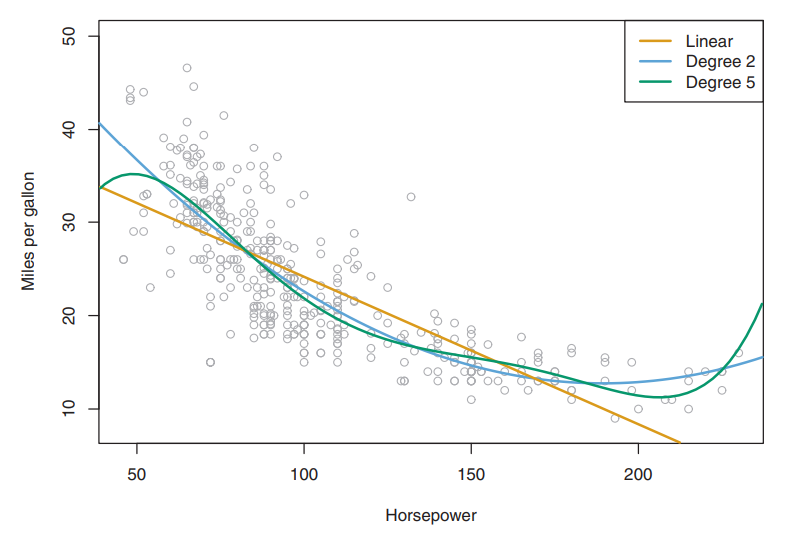
\includegraphics[scale=0.8]{images/pol-reg.png}
\end{center}
Consider the figure above,  in which the mpg (gas mileage in miles per gallon) versus horsepower is shown for a number of cars in the Auto data set. The orange line represents the linear regression fit. There is a pronounced relationship between mpg and horsepower, but it seems clear that this relationship is in fact non-linear: the data suggest a curved relationship. A simple approach for incorporating non-linear associations in a linear model is to include transformed versions of the predictors in the model.\\\\
For example, the points in the figure seem to have a quadratic shape, suggesting that a model of the form
\[mpg = \beta_0 + \beta_1 \times horsepower + \beta_2 \times horsepower^2 + \epsilon\]
may provide a better fit. It involves predicting mpg using a
non-linear function of horsepower. But it is still a linear model! That is, it is simply a multiple linear regression model with $X_1 = horsepower$ and $X_2 = horsepower^2$. So we can use standard linear regression software to estimate $\beta_0, \beta_1$, and $\beta_2$ in order to produce a non-linear fit.\\\\
The blue curve shows the resulting quadratic fit to the data. The quadratic fit appears to be substantially better than the fit obtained when just the linear term is included. The $R^2$ of the quadratic fit is 0.688, compared to 0.606 for the linear fit.\\\\
If including $horsepower^2$ led to such a big improvement in the model, why not include $horsepower^3$, $horsepower^4$, or even $horsepower^5$? The green curve displays the fit that results from including all polynomials up to fifth degree. The resulting fit seems unnecessarily wiggly—that is, it is unclear that including the additional terms really has led to a better fit to the data. 

\subsection{Removing the Additive Assumption}
Consider the standard linear regression model with two variables,
\[Y = \beta_0 + \beta_1 X_1 + \beta_2 X_2 + \epsilon\]
According to this model, if we increase $X_1$ by one unit, then $Y$ will increase by an average of $\beta_1$ units. Notice that the presence of $X_2$ does not alter this statement, that is, regardless of the value of $X_2$, a one-unit increase in $X_1$ will lead to a $\beta_1$-unit increase in $Y$.\\\\
One way of extending this model to allow for interaction effects is to include a third predictor, called an \textit{interaction term}, which is constructed by computing the product of $X_1$ and $X_2$. This results in the model
\[Y = \beta_0 + \beta_1 X_1 + \beta_2 X_2 + \beta_3 X_1X_2 + \epsilon\]
How does inclusion of this interaction term relax the additive assumption? Note that the equation above can be rewritten as
\[Y = \beta_0 +  (\beta_1 + \beta_3X_2)X_1 + \beta_2X_2 + \epsilon\]
Note that the effect of $X_1$ on $Y$ is no longer constant: adjusting $X_2$ will change the impact of $X_1$ on $Y$. For example, suppose that we are interested in studying the productivity of a factory. We wish to predict the number of units produced on the basis of the number of production lines and the total number of workers.\\\\
It seems likely that the effect of increasing the number of production lines will depend on the number of workers, since if no workers are available to operate the lines, then increasing the number of lines will not increase production. This suggests that it would be appropriate to include an interaction term between lines and workers in a linear model to predict units. Suppose that when we fit the model, we obtain
\[
\begin{split}
    units & \approx 1.2+3.4 \times lines + 0.22 \times workers + 1.4 \times (lines \times workers)\\
    & = 1.2 + (3.4+1.4 \times workers) \times lines + 0.22 \times workers.
\end{split}
\]
In other words, adding an additional line will increase the number of units produced by $3.4+1.4 \times workers$. Hence the more workers we have, the stronger will be the effect of lines.\\\\
Consider the Credit data set example we already seen, and suppose that we wish to predict balance using the income (quantitative) and student (qualitative) variables. In the absence of an interaction term, the model takes the form
\[
\begin{split}
    balance_i & \approx \beta_0 + \beta_1 \times income_i + \begin{cases}
    \beta_2 & \text{if $i$-th person is a student}\\
    0 & \text{otherwise}
\end{cases}\\
    & = \beta_1 \times income_i + \begin{cases}
        \beta_0 + \beta_2 & \text{if $i$-th person is a student}\\
        \beta_0 & \text{otherwise}
    \end{cases}
\end{split}
\]
Notice that this amounts to fitting two parallel lines to the data, one for students and one for non-students. The lines for students and non-students have different intercepts, $\beta_0 + \beta_2$ versus $\beta_0$, but the same slope, $\beta_1$.
\begin{center}
    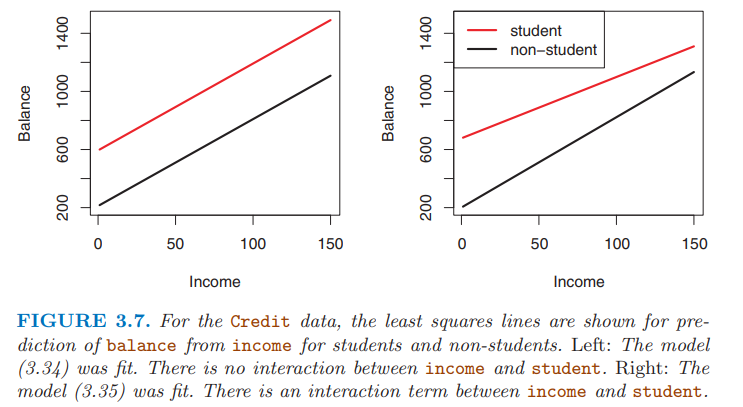
\includegraphics[scale=0.8]{images/creadit card ex. additive.png}
\end{center}
The fact that the lines are parallel means that the average effect on balance of a one-unit increase in income does not depend on whether or not the individual is a student. This represents a potentially serious limitation of the model, since in fact a change in income may have a very different effect on the credit card balance of a student versus a non-student.\\\\
This limitation can be addressed by adding an interaction variable, created by multiplying income with the dummy variable for student. Our model now becomes
\[
\begin{split}
    balance_i & \approx \beta_0 + \beta_1 \times income_i + \begin{cases}
    \beta_2 + \beta_3 \times income_i & \text{if student}\\
    0 & \text{otherwise}
\end{cases}\\
    & = \begin{cases}
        (\beta_0 + \beta_2)+(\beta_1 + \beta_3) \times income_i & \text{if student}\\
        \beta_0 + \beta_1 \times income_i & \text{otherwise}
    \end{cases}
\end{split}
\]
Once again, we have two different regression lines for the students and the non-students. But now those regression lines have different intercepts, $\beta_0+\beta_2$ versus $\beta_0$, as well as different slopes, $\beta_1+\beta_3$ versus $\beta_1$. This allows for the possibility that changes in income may affect the credit card balances of students and non-students differently.\\\\
From the right panel of the figure above we note that the slope for students is lower than the slope for non-students. This suggests that increases in income are associated with smaller increases in credit card balance among students as compared to non-students.

\section{Potential Problems}
When we fit a linear regression model to a particular data set, many problems may occur. Most common among these are the following:
\begin{enumerate}
    \item Non-linearity of the response-predictor relationships.
    \item Correlation of error terms.
    \item Non-constant variance of error terms.
    \item Outliers.
    \item High-leverage points.
    \item Collinearity.
\end{enumerate}

\subsection{Non-linearity of the response-predictor relationships}
The linear regression model assumes that there is a straight-line relationship between the predictors and the response. If the true relationship is far from linear, then virtually all of the conclusions that we draw from the fit are suspect. In addition, the prediction accuracy of the model can be significantly reduced.
\\\\
Residual plots are a useful graphical tool for identifying non-linearity. Given a simple linear regression model, we can plot the residuals, $e_i = y_i - \hat{y}_i$, versus the predictor $x_i$. In the case of a multiple regression model, since there are multiple predictors, we instead plot the residuals versus the predicted (or fitted) values $\hat{y}_i$. Ideally, the residual plot will show no  discernible pattern. The presence of a pattern may indicate a problem with some aspect of the linear model.
\begin{center}
    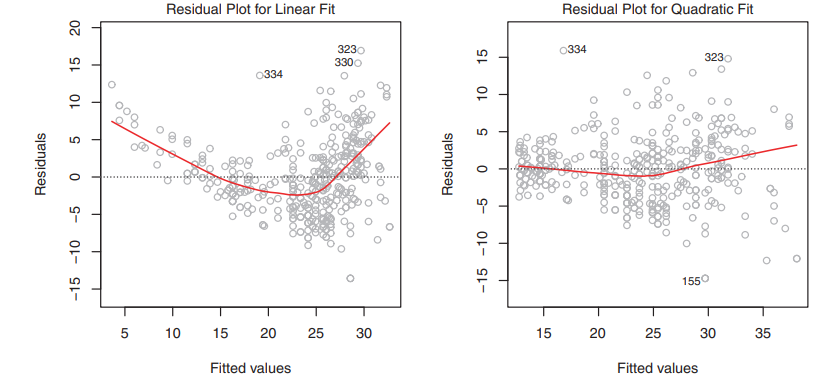
\includegraphics[scale=0.8]{images/residual-plot.png}
\end{center}

\subsection{Correlation of Error Terms}
An important assumption of the linear regression model is that the error terms, $\epsilon_1, \epsilon_2,...,\epsilon_n$, are uncorrelated. What does this mean? For instance, if the errors are uncorrelated, then the fact that $\epsilon_i$ is positive provides little or no information about the sign of $\epsilon_{>i+1}$. The standard errors that are computed for the estimated regression coefficients or the fitted values are based on the assumption of uncorrelated error terms. However, if the error terms are correlated, we may have an unwarranted sense of confidence in our model. Such correlations frequently occur in the context of time series data, which consists of observations for which measurements are obtained at discrete points in time.

\subsection{Non-constant Variance of Error Terms}
Another important assumption of the linear regression model is that the error terms have a constant variance, $\text{Var}(\epsilon_i) = \sigma^2$. The standard errors, confidence intervals, and hypothesis tests associated with the linear model rely upon this assumption.\\\\
Unfortunately, it is often the case that the variances of the error terms are non-constant. For instance, the variances of the error terms may increase with the value of the response. One can identify non-constant variances in the errors, or heteroscedasticity, from the presence of a funnel shape in the residual plot.
\begin{center}
    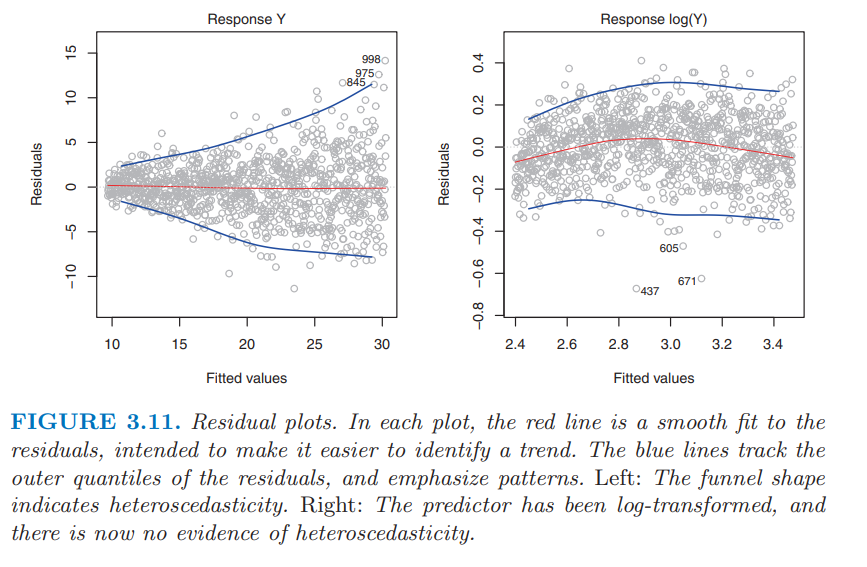
\includegraphics[scale=0.8]{images/non-const-var.png}
\end{center}
When faced with this problem, one possible solution is to transform the response $Y$ using a concave function such as $log \,\,Y$ or $\sqrt{Y}$ . Such a transformation results in a greater amount of shrinkage of the larger responses, leading to a reduction in heteroscedasticity.

\subsection{Outliers}
An outlier is a point for which $y_i$ is far from the value predicted by the model. Outliers can arise for a variety of reasons, such as incorrect recording of an observation during data collection.\\\\
 It is typical for an outlier that does not have an unusual
predictor value to have little effect on the least squares fit. However, even if an outlier does not have much effect on the least squares fit, it can cause other problems. For example, it can drastically affect the RSE or $R^2$ statistics. Since the RSE is used to compute all confidence intervals and p-values, such a dramatic increase caused by a single data point can have implications for the interpretation of the fit. If we believe that an outlier has occurred due to an error in data collection or recording, then one solution is to simply remove the observation. However, care should be taken, since an outlier may instead indicate a deficiency with the model, such as a missing predictor.

\subsection{High Leverage Points}
We just saw that outliers are observations for which the response $y_i$ is unusual given the predictor $x_i$. In contrast, observations with high leverage have an unusual value for $x_i$.
\begin{center}
    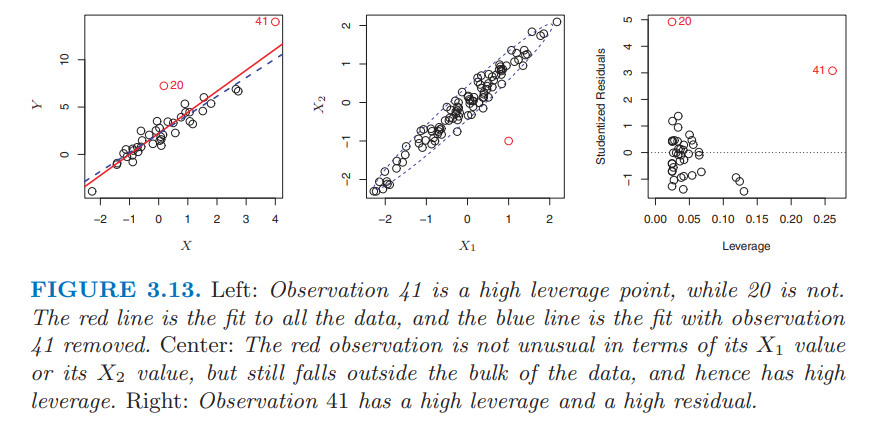
\includegraphics[scale=0.8]{images/high-laverage.png}
\end{center}
Removing the high leverage observation has a much more substantial impact on the least squares line than removing the outlier. In fact, high leverage observations tend to have a sizable impact on the estimated regression line. It is cause for concern if the least squares line is heavily affected by just a couple of observations,
because any problems with these points may invalidate the entire fit. For this reason, it is important to identify high leverage observations.

\subsection{Collinearity}
Collinearity refers to the situation in which two or more predictor variables are closely related to one another. The presence of collinearity can pose problems in the regression context, since it can be difficult to separate out the individual effects of collinear variables on the response.\\\\
Since collinearity reduces the accuracy of the estimates of the regression coefficients, it causes the standard error for $\hat\beta_j$ to grow. Recall that the t-statistic for each predictor is calculated by dividing $\hat\beta_j$ by its standard error. Consequently, collinearity results in a decline in the t-statistic. As a result, in the presence of collinearity, we may fail to reject $H0 : \beta_j = 0$.\\\\
A simple way to detect collinearity is to look at the correlation matrix of the predictors. An element of this matrix that is large in absolute value indicates a pair of highly correlated variables, and therefore a collinearity problem in the data. Unfortunately, not all collinearity problems can be detected by inspection of the correlation matrix: it is possible for collinearity to exist between three or more variables even if no pair of variables has a particularly high correlation. We call this situation \textit{multicollinearity}.
